% !TEX root = ../dg.tex

\section{Gradients and Optimization}
\label{sec:gradients}

In practical problems, we are very often interested in minimizing (or maximizing) some function $f \from M \to \R$. 

\begin{example}\label{ex:frame potential}
If $n > d$ and I take $M = (S^{d-1})^n$, then I can interpret $(x_1, \dots , x_n) \in M$ as a collection of unit vectors in $\R^d$ and hence, so long as the vectors $x_1, \dots , x_n$ form a spanning set for $\R^d$, a \emph{unit-norm frame} in $\R^d$. We will also package the $x_i$ into a $d \times n$ matrix $X = \begin{bmatrix} x_1 & \dots & x_n\end{bmatrix}$. Define the function $\FP \from M \to \R$ by
\[
	\FP(X) := \|XX^\ast\|_{\text{Fr}}^2,
\]
where the norm is the Frobenius norm. This function is usually called the \emph{frame potential}, and it is a straightforward exercise to show that the global minima of $\FP$ are the so-called \emph{unit-norm tight frames}. A celebrated theorem of Benedetto and Fickus~\cite{benedettoFiniteNormalizedTight2003} says that all local minima of this function are global, so there is no danger of getting trapped in a local minimum when trying to optimize this function.
\end{example}


Of course, the most naïve way of minimizing a function is to do gradient descent: that is, to flow in the direction of the negative gradient. But that raises the question: what is the gradient on a manifold, and does gradient descent still make sense?

I have already implicitly addressed the first question in \Cref{sec:vector calculus}, but let's make that discussion clearer and more explicit. The first thing to do is to recall a useful characterization of the gradient of a function $f \from \R^n \to \R$: for a tangent vector $v$, 
\begin{equation}\label{eq:euclidean gradient}
	\nabla f(p) \cdot v = \frac{\partial f}{\partial v}(p);
\end{equation}
that is, the dot product of the gradient of $f$ with any tangent vector $v$ gives the directional derivative of $f$ in the direction of $v$.

We now have all the machinery in place to interpret everything in \Cref{eq:euclidean gradient} on manifolds. For the left hand side, we should think of $\nabla f(p)$ and $v$ as elements of $T_pM$, and then a Riemannian metric $g$ tells us the inner product on $T_pM$, so the left-hand side becomes $g_p(\nabla f(p), v)$. In fact, I'm going to use $\grad f$ rather than $\nabla f$ for the gradient on manifolds, since we're already using $\nabla$ for the Levi-Civita connection, so the left-hand side is really going to be $g_p(\grad f(p), v)$. 

For the right-hand side of \Cref{eq:euclidean gradient}, recall that way back in \Cref{sec:tangent vectors} we defined tangent vectors as directional derivative operators, so the right way of saying $\frac{\partial f}{\partial v}$ is $v(f)$.

In other words, we can get a generalization of \Cref{eq:euclidean gradient} to arbitrary Riemannian manifolds by writing
\begin{equation}\label{eq:grad1}
	g_p(\grad f(p), v) = v(f).
\end{equation}
In fact, if we recall \Cref{lem:vector fields and differentials}, we know that $v(f) = df_p(v)$ is just the differential of $f$ evaluated on $v \in T_p M$. So we can also write
\begin{equation}\label{eq:grad2}
	g_p(\grad f(p), v) = df_p(v)
\end{equation}
for any $v \in T_pM$. This will be, in fact, the definition of the gradient we give below in \Cref{def:gradient}, but let's put this in a slightly more general framework first (building on the informal discussion in \Cref{sec:vector calculus}).

Say that $f \from M \to \R$ is a smooth function. Then the differential $df \in \Omega^1(M)$ is a 1-form. Moreover, if $M$ is not just a manifold but a Riemannian manifold, then I can use the Riemannian metric to identify 1-forms with vector fields. 

More precisely, for any 1-form $\omega \in \Omega^1(M)$, define $\omega^\sharp \in \mathfrak{X}(M)$ by
\[
	g_p(\omega^\sharp(p),v) = \omega_p(v)
\]
for any $v \in T_pM$. For each $p \in M$ we know there is such a vector $\omega^\sharp(p) \in T_pM$ by the Riesz Representation Theorem, and the fact that $\omega^\sharp$ is smooth follows from the smoothness of $g$ and $\omega$. 

More abstractly, we could write
\[
	g(\omega^\sharp,\cdot) = \omega.
\]
In local coordinates, we have that $\omega = \sum_i w_i dx^i$ and any $v = \sum_i v^i \frac{\partial}{\partial x_i}$, so
\[
	\omega_p(v) = \left( \sum_i w_i dx^i\right) \left( \sum_i v^i \frac{\partial}{\partial x_i} \right) = \sum_i w_iv^i.
\]
On the other hand, $\omega^\sharp = \sum_i u^i \frac{\partial}{\partial x_i}$ and
\[
	g_p(\omega^\sharp(p),v) = g_p\left(\sum_i u^i \frac{\partial}{\partial x_i}, \sum_i v^i \frac{\partial}{\partial x_i} \right) = \sum_{i,j} u^i v^j g_{ij}.
\]
Equating coefficients gives
\[
	w_i = \sum_j u^j g_{ij}
\]
or
\[
	u^j = \sum_i w_i g^{ij}.
\]

Putting this together, then, we have that for $\omega = \sum_i w_i dx^i$, the dual vector field is
\begin{equation}\label{eq:raising indices}
	\omega^\sharp = \sum_{i,j} w_i g^{ij} \frac{\partial}{\partial x_j}.
\end{equation}

When we let $\omega = df$, the resulting vector field is the gradient:

\begin{definition}\label{def:gradient}
	If $(M,g)$ is a Riemannian manifold and $f \from M \to \R$ is smooth, then the \emph{gradient} of $f$ is the vector field $\grad f = (df)^\sharp \in \mathfrak{X}(M)$.
\end{definition}

If we just unwind the definitions and recall \Cref{lem:vector fields and differentials}, we see that, for any $X \in \mathfrak{X}(M)$,
\[
	g(\grad f, X) = df(X) = Xf,
\]
as in \eqref{eq:grad1} and \eqref{eq:grad2}.

In coordinates, we know that 
\[
	df = \sum_i \frac{\partial f}{\partial x_i} dx^i,
\]
so \eqref{eq:raising indices} tells us that
\[
	\grad f = \sum_{i,j} \frac{\partial f}{\partial x_i} g^{ij} \frac{\partial}{\partial x_j}.
\]

\begin{example}
	Suppose $M=\R^n$ with the standard Euclidean metric. Then $g^{ij} = \delta^{ij}$, so we see that
	\[
		\grad f = \sum_{i,j} \frac{\partial f}{\partial x_i} \delta^{ij} \frac{\partial}{\partial x_j} = \sum_i \frac{\partial f}{\partial x_i} \frac{\partial}{\partial x_i}
	\]
	is the usual gradient you learned in multivariable calculus.
\end{example}

\begin{example}
	Let $M = \Aff^+(\R) \cong H$ with the Riemannian metric from \Cref{ex:affine hyperbolic metric}; that is, $g_{11} = \frac{1}{y^2} = g_{22}$ and $g_{12} = 0$. Then $g^{11} = y^2 = g^{22}$ and $g^{12} = 0$, so we have
	\[
		\grad f = y^2 \left(\frac{\partial f}{\partial x} \frac{\partial}{\partial x} + \frac{\partial f}{\partial y} \frac{\partial}{\partial y} \right)
	\]
	looks like the Euclidean gradient scaled by $y^2$.
\end{example}

\begin{example}
	Let $M = S^1$ with its standard Riemannian metric $g\left(\frac{\partial}{\partial \theta},\frac{\partial}{\partial \theta}\right) = 1$; that is $g = \begin{bmatrix}g_{11} \end{bmatrix} = \begin{bmatrix} 1 \end{bmatrix}$, so $g^{11} = 1$ and we have
	\[
		g\left(\grad f, \frac{\partial}{\partial \theta}\right) df\left( \frac{\partial}{\partial \theta} \right) = \frac{\partial }{\partial \theta} f.
	\]
	If I think of $S^1 \subset \R^2$, then I can interpret $\frac{\partial}{\partial \theta} \in T_{\theta} S^1 \subset T_{(\cos \theta,\sin \theta)} \R^2$ as a tangent vector to $\R^2$, namely as 
	\[
		\frac{\partial}{\partial \theta} = y \frac{\partial}{\partial x} -x \frac{\partial}{\partial y}.
	\]
	So in Cartesian coordinates,
	\[
		\frac{\partial }{\partial \theta} f = \left(y \frac{\partial}{\partial x} -x \frac{\partial}{\partial y} \right) = y \frac{\partial f}{\partial x} - x \frac{\partial f}{\partial y} = (\nabla f) \cdot \left( y\frac{\partial}{\partial x} - x\frac{\partial}{\partial y}\right),
	\]
	where $\grad f$ is the gradient of $f$ in $\R^2$ and $\cdot $ is the usual Euclidean dot product. But now
	\[
		(\nabla f) \cdot \left( y\frac{\partial}{\partial x} - x\frac{\partial}{\partial y}\right) \frac{\partial}{\partial \theta}
	\]
	is just the orthogonal projection of $\nabla f$ onto the tangent space to $S^1$.
	
	In other words, at least in this case, we can compute $\grad f$ by computing the extrinsic Euclidean gradient and then projecting onto the tangent space to the submanifold we're interested in.
\end{example}

In fact, this is true more generally:

\begin{proposition}\label{prop:gradient projection}
	Let $(M,\overline{g})$ be a Riemannian manifold, $N \subset M$ a smooth submanifold with its induced Riemannian metric $g$, and $\overline{f} \from M \to \R$ a smooth function. Let $f \from N \to \R$ be the restriction of $\overline{f}$ to $N$; that is, $f = \left. \overline{f} \right|_N$. If we let $\overline{\grad f}$ be the gradient of $\overline{f}$ in $M$, and $\grad f$ the gradient of $f$ in $N$, then at each point $p \in N$ the gradient $\grad f$ is the orthogonal projection of $\overline{\grad f}$ to the tangent space $T_pN \subset T_pM$.
\end{proposition}

\begin{proof}
	Let $\iota \from N \to M$ be the inclusion map. Then $f = \overline{f} \circ \iota$, and hence
	\[
		\iota^\ast \left(d\overline{f}\right) = d \left(\iota^\ast \overline{f}\right) = d\left(\overline{f} \circ \iota\right) = df
	\]
	by \Cref{prop:pullbacks commute with exterior derivative}. Therefore, for any $v \in T_pN$,

	\[
		g_p(\grad f, v) = df_p(v) = \left(\iota^\ast\left(d \overline{f}\right)\right)(v) = d\overline{f}_p(d\iota_p v) =\overline{g}_p(\overline{\grad f},d\iota_p v).
	\]
	Of course, $d\iota_p \from T_pN \to T_p M$ is just the inclusion map so
	\[
		g_p(\grad f, v) = \overline{g}_p(\overline{\grad f},v).
	\]
	The only vector which satisfies this equation for all $v \in T_pN$ is the orthogonal projection of $\overline{\grad f}$ onto $T_pN$.
\end{proof}

In particular, when $N \subset \R^n$ is a smooth submanifold, then the Riemannian gradient $\grad f$ at a point $p$ is simply the orthogonal projection of the usual Euclidean gradient $\nabla f$ onto $T_pN$. In many cases (spheres, Stiefel manifolds, etc.) we are interested in smooth submanifolds of Euclidean space and so we can compute gradients in this fairly straightforward way.

Note that the Riemannian gradient has the same interpretation as the direction of steepest ascent:

\begin{proposition}\label{prop:gradient steepest ascent}
	Let $(M,g)$ be a Riemannian manifold, $f \from M \to \R$ smooth, and $p \in M$ a regular point of $f$. Among all unit vectors $v \in T_pM$, the directional derivative $v(f)$ is greatest when $v$ points in the direction of $\grad f$ and $\|\grad f\|$ is equal to the value of the directional derivative in that direction.
\end{proposition}

\begin{proof}
	If $v \in T_pM$ is any unit vector, the Cauchy–Schwarz inequality says that
	\[
		v(f) = g_p(\grad f, v) \leq \|\grad f\|\|v\|
	\]
	with equality if and only if $\grad f$ and $v$ point in the same direction. 
	
	When $\grad f$ and $v$ point in the same direction,
	\[
		v(f) = \|\grad f\|\|v\| = \|\grad f\|
	\]
	since $\|v\| = 1$.
\end{proof}

Also, just as in Euclidean space, the gradient of a function is perpendicular to level sets of the function.

\begin{proposition}\label{prop:gradient normal to level sets}
	Let $(M,g)$ be a Riemannian manifold, $f \from M \to \R$ smooth, and $p \in M$ a regular point of $f$. Then $\grad f$ is perpendicular to the level set of $f$ through $p$.
\end{proposition}

\begin{exercise}
	Prove \Cref{prop:gradient normal to level sets}.
\end{exercise}

For $f \from M \to \R$ smooth, we've now seen that $\grad f \in \mathfrak{X}(M)$. Then the \emph{gradient flow} of $f$ is simply the local flow of the vector field $\grad f$. We can also pose this as an ODE:

\begin{definition}\label{def:negative gradient flow}
	Let $(M,g)$ be a Riemannian manifold, $f \from M \to \R$ smooth, and $p_0 \in M$. Then the \emph{negative gradient flow} of $f$ starting at $p_0$ is the map $\Gamma \from M \times [0,T) \to M$ defined by
	\[
		\Gamma(p_0,0) = p_0, \qquad \frac{d}{dt}\Gamma(p_0,t) = -\grad f(\Gamma(p_0,t)),
	\]
	where $T \in (0,+\infty]$ is some time after which the flow may cease to exist.
\end{definition}
By the usual existence and uniqueness theorems of ODEs, this is well-defined and has a unique solution for all $t$ sufficiently small.

Bringing this back to \Cref{ex:frame potential}, Dustin Mixon, Tom Needham, Soledad Villar and I~\cite{mixonThreeProofsBenedetto2023} proved that for almost every $F_0 \in M$, the negative gradient flow of $\FP$ starting at $F_0$ exists for all time and limits, as $t \to +\infty$, to a unit-norm tight frame; that is, a global minimizer of $\FP$. This is true in spite of the fact that the frame potential $\FP$ is not convex: indeed, it has lots of non-minimizing critical points.

Numerically, how can we actually do gradient descent? Well, at each point $p$ we want to move in the direction of the vector $-\grad f(p)$. But we know how to do this (at least in principle): use the Riemannian exponential map! So an algorithm for Riemannian gradient descent looks something like this:

\ifplastex
	\begin{center}
		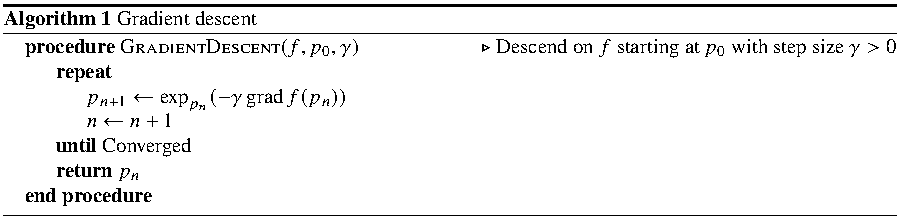
\includegraphics[height=2in]{alg1}
	\end{center}
\else
	\begin{algorithm}[H]
	%\capstart
	\begin{algorithmic}
	\Procedure{GradientDescent}{$f,p_0,\gamma$}\Comment{Descend on $f$ starting at $p_0$ with step size $\gamma > 0$}
	\Repeat
		\State $p_{n+1} \gets \exp_{p_n}(-\gamma \grad f(p_n))$
		\State $n \gets n+1$
	\Until{Converged}
	\Return{$p_n$}
	\EndProcedure
	\end{algorithmic}
	\caption{Gradient descent}
	\label{alg:gradient descent}
	\end{algorithm}
\fi

Of course, computing the Riemannian exponential map generally involves solving the geodesic equation, which is a second-order ODE, so as stated \ifplastex Algorithm 1 \else \Cref{alg:gradient descent so(n)} \fi is not usually very practical. The typical strategy for doing gradient descent in practice is to find some approximation to the exponential map which is well-adapted to the manifold of interest. 

For example, if $M \subset \R^n$ is a smooth submanifold, then for small $\gamma > 0$, $\exp_p(\gamma v)$ will be very close to the point in $M$ which is closest to $p + \gamma v \in \R^n$. Hence, if there is a good way of projecting a point in $\R^n$ back to $M$, we can replace $\exp_{p_n}(-\gamma \grad f(p_n))$  in \ifplastex Algorithm 1 \else \Cref{alg:gradient descent so(n)} \fi with the result of applying this projection to $p_n - \gamma \grad f(p_n) $.

\begin{example}
	Consider $\SO(n) \subset \Mat_{n \times n}(\R)$. Then for a function $f \from \SO(n) \to \R$ with a smooth extension to (a neighborhood of $\SO(n)$ in) $ \Mat_{n \times n}(\R)$, we can approximate the gradient descent of $f$ as in \ifplastex Algorithm 2 \else \Cref{alg:gradient descent so(n)} \fi. 
	
	
\ifplastex
	\begin{center}
		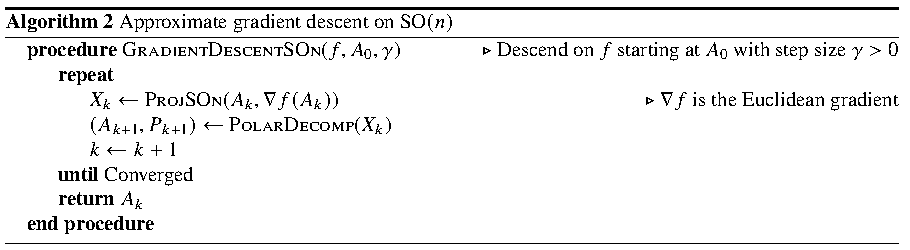
\includegraphics[height=2in]{alg2}
	\end{center}
\else
	\begin{algorithm}[H]
	%\capstart
	\begin{algorithmic}
	\Procedure{GradientDescentSOn}{$f,A_0,\gamma$}\Comment{Descend on $f$ starting at $A_0$ with step size $\gamma > 0$}
	\Repeat
		\State $X_{k} \gets $ \Call{ProjSOn}{$A_k,\nabla f(A_k)$}\Comment{$\nabla f$ is the Euclidean gradient}
		\State $(A_{k+1}, P_{k+1}) \gets $ \Call{PolarDecomp}{$X_k$}
		\State $k \gets k+1$
	\Until{Converged}
	\Return{$A_k$}
	\EndProcedure
	\end{algorithmic}
	\caption{Approximate gradient descent on $\SO(n)$}
	\label{alg:gradient descent so(n)}
	\end{algorithm}
\fi
	
	This depends on two functions, {\sc ProjSOn} and {\sc PolarDecomp}, defined as follows.
		\begin{itemize}
			\item For $A \in \SO(n)$ and $X \in \Mat_{n \times n}(\R)$, {\sc ProjSOn}$(A,X)$ is the orthogonal projection of $X$ to 
		\[
			T_A \SO(n) = \{A \Delta : \Delta \in \Mat_{n \times n}(\R) \text{ is skew-symmetric}\}.
		\]
	
		\item For $X \in \Mat_{n \times n}(\R)$, {\sc PolarDecomp}$(X)$ returns the pair $(U,P)$, where $X = UP$ is the polar decomposition of $X$. Note that $U$ is the closest matrix in $\SO(n)$ to $X$.\footnote{For more on the geometry and topology of matrix decompositions, see~\cite{deturckMakingMatricesBetter2017b}.}
		\end{itemize}
\end{example}

